\section{kill.c}

	Muestre la pantalla de ejecución del programa.

	\begin{center}
		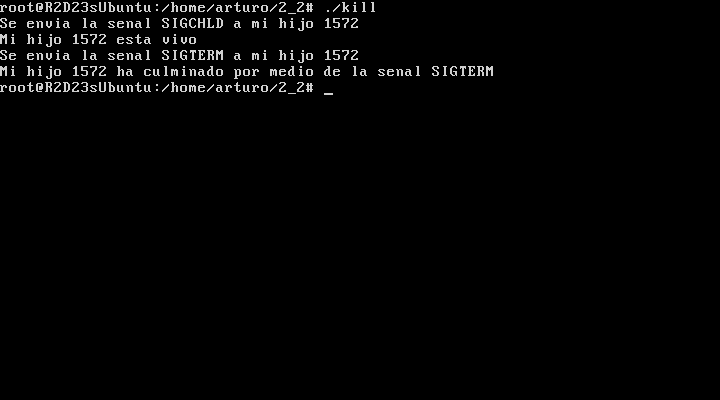
\includegraphics[width=\linewidth]{imagenes/kill.png}
	\end{center}

	Describa cuál es el propósito de las siguientes bibliotecas:

	\begin{itemize}

		\item signal.h
	\begin{tcolorbox}
		Esta biblioteca es utilizada para manejar señales.
	\end{tcolorbox}
		\item stdlib.h
	\begin{tcolorbox}
		Biblioteca estándar que utilizamos para manejar los procesos. Nos define las macros EXIT\_SUCCESS y EXIT\_FAILURE y la función \textit{exit()}.
	\end{tcolorbox}

	\end{itemize}

	Para las siguientes funciones, mencione dónde están definidas, qué es lo que proporcionan de salida y qué argumentos necesitan de entrada:

	\begin{itemize}

		\item exit
	\begin{tcolorbox}
		Está definida en la biblioteca \textit{stdlib.h}. No regresan nada y requieren un entero que representará el estado de salida del proceso. Termina el proceso.
	\end{tcolorbox}
		\item kill
	\begin{tcolorbox}
		Está definida en la biblioteca \textit{signal.h}. Regresa 0 si tuvo éxito, -1 si falló. Pide como parámetros la señal a enviar y el pid del proceso a enviar la señal. Si es > 0, se enviará la señal al proceso específico. Igual a 0 enviará la señal a todos los procesos del grupo del emisor. -1 enviará la señal a todos los procesos.
	\end{tcolorbox}

	\end{itemize}

	Mencione el significado de los siguientes valores de salida en exit:

	\begin{itemize}

		\item EXIT SUCCESS
	\begin{tcolorbox}
		El valor a regresar si el proceso ha acabado con éxito.
	\end{tcolorbox}
		\item EXIT FAILURE
	\begin{tcolorbox}
		El valor a regresar si el proceso ha acabado con errores.
	\end{tcolorbox}

	\end{itemize}